\chapter{Method}
To be able to re-engineer MediaSense it is necessary to rethink and re-design core-components of the an existing middleware. Using traditional quantitative or qualitative research methods would not involve any actual design. These research methods produce data based on past or present conditions and are usually not used to develop artefacts.
Design science research differs in one major way from qualitative or quantitative empirical studies. Where empirical studies focus on finding patterns in the past or present state of an industry or a field, design science is intended to design and develop new solutions to actual problems \cite{bider2012design} and aims to improve and create artefacts that can improve the world \cite{johannesson2012design}. Because the re-engineering MediaSense means re-designing an artefact design science reasearch is pertinent for the task.
Design science involves consists of a few steps, or actions. The first action is to explicate the problem, the second is identifying requirements and the third is a design and develop action where an artefact is constructed based on the requirements previously identifyed. An optional demonstration action can be applied to show the artefact in a real life scenario. Lastly there is an evaluation action where the artefact is evaluated based on the requirements to see if they have been met and thus if the artefact solved the problem. Consequently design science is a good method to use for this problem where a redesign of an existing middleware for the Internet of Things is needed.

\begin{figure}[h!]
	\centering
    	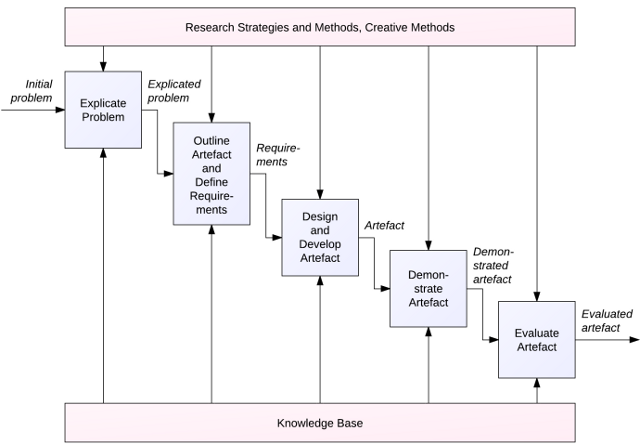
\includegraphics[scale=0.50]{part_3/design_science.png}
		\caption{Diagram of the Design Science Method \cite{johannesson2012design}} 
		\label{ds}
\end{figure}

The method chosen for this research is design science as defined by Johannesson and Perjons in A Design science primer \cite{johannesson2012design}. It is well structured and has guidelines that makes it easy to use as opposed to other definitions of design science such as the one laid out in Memorandum on design-oriented information systems research \cite{osterle2010memorandum} or the one mentioned in Design science in information systems research \cite{hevner2004design}. Johannesson and Perjons mention that Design Science consists of 5 actions, as shown in figure \ref{ds}. These actions are carried out iteratively instead of sequentially because later actions can yeild information necessary to previous actions, i.e., the design and develop action reveals new requirements for the artefact. In design science it is possible to use other methods to answer questions about artefact. Every action in Figure \ref{ds} should have its own research strategy and methods. For this thesis the demonstration action will be omitted. MediaSense is still a research project and real life use-cases for the demonstration would require actual applications. The evaluation action will include tests with test applications that sufficiently demonstrate that the problem has been solved.

\section{Research Strategies and Methods}
\section{Research method for Explicate Problem}
To explicate the problem we chose to do a document study of previous publications regarding internet of things middleware. The document study also considered of reading the source code for MediaSense to get an insight into how MediaSense is constructed and how it worked. Combining this method with interviews of a person with more knowledge about the concept internet of things and knowledge about MediaSense helped to explicate the problem and give a broader knowledge base of the surrounding concepts for internet of things middleware. With a broader knowledge base the problem can then be broken down into a number of subproblems. 

An alternative to these methods could be survey using questionnaires, in which predefined written questions can be asked to a respondent. This method can easy be distributed to a large number of respondents. It was not chosen because the researcher cannot ask follow up questions which makes it hard to discuss a problem situation and because there are few persons with knowledge about MediaSense the result of a questionnaire would not explicate the problem, especially when follow up questions is not possible. If there was a larger group of stakeholders for MediaSense a survey could have been used to explicate the problem, but this was not the case and surveys was excluded.

\section{Research Method For Define Requirements}
Due to there only being one stakeholder with sufficient knowledge of MediaSense and as such quantitative methods are not applicable for defining the requirements of the artefact.
The qualitative methods we considered were observation, case study, interview and group discussions. To perform an observational study we would need a subject to observe in its natural environment but distributed Internet of Things middleware is still a subject of research and as such the intended environment does not yet exist. Conducting group discussions is not applicable in our situation because there only is one stakeholder.
Interviews at first seemed like a good approach because there only is one very involved stakeholder with whom we can conduct the interviews and thus get a deep understanding of the stakeholders needs. A problem with interviews is that the reliability or validity of the answers isn't guaranteed \cite{golafshani2003understanding}, even though the respondent might answer to their best ability it is possible that not all requirements are immediately unearthed due to the restricted perspectives. Interviews also tend to stifle creativity and are dependent on the questions asked \cite{johannesson2012design} thus resulting in important requirements being missed. Because the stakeholder also was responsible for the artefact the answers given in an interview could be coloured by his own view of the artefact.
A case study with both interviews and a deeper study of the artefact was then the best solution as this would make it possible to determine how aspects of the artefact worked before conducting unstructured and open-ended interviews to determine how the solution should work.


\section{Research For Design And Develop Artefact}
With the information gathered in the earlier stages of the design science process architectural changes will need to be designed. For this process participative modelling \cite{johannesson2012design} and document study will be used. The participative modelling will mainly be done by drawing architectural models on a whiteboard and the document studies will be done to research similar solutions and usable technologies. 

The development of the design will be done with pair programming \cite{williams2000all} which is a practice from the software development methodology extreme programming. According to  \cite{williams2000all} two programmers working together will find twice as many solutions to a problem than working alone. Also bugs will be found in an earlier state and this will give higher quality on the artefact. 

\subsection{Evaluate Artefact}
To evaluate the artifact it is necessary to validate that the requirements gathered in the earlier action \emph{defining requirements}, have been met. The strategies considered for evaluation are Surveys, Experiments, Case studies, Ethnography, Theoretical Analysis. 
Doing an ethnographic study would give valuable insights into how an Internet of Things platform would be used and how our redesign would impact usage. Given that Internet of Things still isn't a widely adopted paradigm there would be no precedent to compare cultural impacts to. Such a study would only contribute to the understanding of how people use the Internet of Things and not our artifact specifically. A case study allows for a deep study of the artefact but can be biased by the researchers perceptions, thus doing a case study of an artifact we ourselves developed will be inconclusive as to if the artifact fulfils the requirements.
Experiments allow us to set up an artificial scenario similar to that in the demonstration. The experiment will be designed to specifically validate all the requirements. A drawback to using experiments is that the artificial scenario doesn't reflect a real life scenario. To rectify this we will use Theoretical analysis of the results from the experiment. Thus we chose to evaluate the artifact with experiments and theoretical analysis.


\section{Ethical Considerations}
All information uncovered in the interviews will be used confidentially and we will assure the respondent consensually agree to have all answers published in this thesis.
The MediaSense platform uses the GNU Lesser General Public License, version 3 \cite{gnu} and as such, there is no confidentiality we need to observe regarding the source code of it.
All test environments used for testing the distributed Internet of Things middleware will be run on a local sandbox for development so the nodes in the network will only contain our own computers. 